\appendix

\part*{ANEXOS}
\addcontentsline{toc}{part}{ANEXOS}
\refstepcounter{part} 

\chapter{A}
\section{A1}
\label{appendix:a}
\begin{longlisting}
	\lstinputlisting{testes/tp1_nc.txt}
	\caption{cópia do ficheiro de dados `tp1\_nc.xls' após ter gerado os valores}
	\label{listing:1}
\end{longlisting}
\section{A2}
\begin{longlisting}
	\lstinputlisting{testes/tp1_ta.txt}
	%\inputminted{text}{./testes/tp1_ta.txt}
	\caption{cópia do ficheiro de dados `tp1\_ta.xls' após ter gerado os valores}
	\label{listing:2}
\end{longlisting}
\section{A3}
\subsection{Tabelas de resultados para o cálculo dos tempos médios de atendimento }
\label{appendix:c1}
\begin{table}[htpb]
\begin{center}
\begin{tabular}{c c c}
\toprule
Frequência & T.\ de atendimento s (segundos) & T.\ de atendimento p/ vol.\
compra\\
\midrule
67 & 28,6 & 1916,2 \\ 
71 & 31,7 & 2250,7 \\ 
88 & 34,8 & 3062,4 \\ 
81 & 37,9 & 3069,9 \\ 
82 & 41   & 3362   \\ 
96 & 44,1 & 4233,6 \\ 
98 & 47,2 & 4625,6 \\ 
88 & 50,3 & 4426,4 \\ 
91 & 53,4 & 4859,4 \\ 
102 & 56,5 & 5763  \\ 
\bottomrule
\end{tabular}
\end{center}
\caption{Listagem freq., tempos de atendimento}
\label{tab:tabela5}
\end{table}


  
\newpage
\begin{longtable}[htpb]{@{}cccc@{}}
\toprule
Nº de artigos& Freq.\ & T.\ de atendimento& T. de atendimento total\\ 
p/ compra &~& s (segundos) & p/ vol.\ de compras \\ 
\midrule
11 & 89   & 59,6  & 5304,4  \\ 
12 & 89   & 62,7  & 5580,3  \\ 
13 & 64   & 65,8  & 4211,2  \\ 
14 & 76   & 68,9  & 5236,4  \\ 
15 & 74   & 72    & 5328    \\ 
16 & 90   & 75,1  & 6759    \\ 
17 & 83   & 78,2  & 6490,6  \\ 
18 & 120  & 81,3  & 9756    \\ 
19 & 100  & 84,4  & 8440    \\ 
20 & 95   & 87,5  & 8312,5  \\ 
21 & 106  & 90,6  & 9603,6  \\ 
22 & 104  & 93,7  & 9744,8  \\ 
23 & 122  & 96,8  & 11809,6 \\ 
24 & 109  & 99,9  & 10889,1 \\ 
25 & 144  & 103   & 14832   \\ 
26 & 140  & 106,1 & 14854   \\ 
27 & 122  & 109,2 & 13322,4 \\ 
28 & 156  & 112,3 & 17518,8 \\ 
29 & 159  & 115,4 & 18348,6 \\ 
30 & 146  & 118,5 & 17301   \\ 
31 & 156  & 121,6 & 18969,6 \\ 
32 & 170  & 124,7 & 21199   \\ 
33 & 183  & 127,8 & 23387,4 \\ 
34 & 185  & 130,9 & 24216,5 \\ 
35 & 201  & 134   & 26934   \\ 
36 & 187  & 137,1 & 25637,7 \\ 
37 & 197  & 140,2 & 27619,4 \\ 
38 & 187  & 143,3 & 26797,1 \\ 
39 & 206  & 146,4 & 30158,4 \\ 
40 & 204  & 149,5 & 30498   \\ 
41 & 206  & 152,6 & 31435,6 \\ 
42 & 199  & 155,7 & 30984,3 \\ 
43 & 196  & 158,8 & 31124,8 \\ 
44 & 242  & 161,9 & 39179,8 \\ 
45 & 220  & 165   & 36300   \\ 
46 & 225  & 168,1 & 37822,5 \\ 
47 & 243  & 171,2 & 41601,6 \\ 
48 & 263  & 174,3 & 45840,9 \\ 
49 & 257  & 177,4 & 45591,8 \\ 
50 & 227  & 180,5 & 40973,5 \\ 
51 & 213  & 183,6 & 39106,8 \\ 
52 & 213  & 186,7 & 39767,1 \\ 
53 & 203  & 189,8 & 38529,4 \\ 
54 & 203  & 192,9 & 39158,7 \\ 
55 & 202  & 196   & 39592   \\ 
56 & 203  & 199,1 & 40417,3 \\ 
57 & 175  & 202,2 & 35385   \\ 
58 & 176  & 205,3 & 36132,8 \\ 
59 & 172  & 208,4 & 35844,8 \\ 
60 & 145  & 211,5 & 30667,5 \\ 
61 & 164  & 214,6 & 35194,4 \\ 
62 & 145  & 217,7 & 31566,5 \\ 
63 & 113  & 220,8 & 24950,4 \\ 
64 & 100  & 223,9 & 22390   \\ 
65 & 129  & 227   & 29283   \\ 
66 & 110  & 230,1 & 25311   \\ 
67 & 95   & 233,2 & 22154   \\ 
68 & 98   & 236,3 & 23157,4 \\ 
69 & 86   & 239,4 & 20588,4 \\ 
70 & 85   & 242,5 & 20612,5 \\ 
71 & 68   & 245,6 & 16700,8 \\ 
72 & 72   & 248,7 & 17906,4 \\ 
73 & 54   & 251,8 & 13597,2 \\ 
74 & 45   & 254,9 & 11470,5 \\ 
75 & 122  & 258   & 31476   \\ \bottomrule
\caption{Listagem freq., tempos de atendimento}
\label{tab:tabela6}
\end{longtable}



\subsection{Resultados obtidos com o \emph{supositorio.com}}
\label{appendix:c2}
\begin{figure}[H]
\centering
\resizebox{0.7\textwidth}{!}{%
\begin{tikzpicture}
	\begin{semilogyaxis}
		    [
					x tick label style={/pgf/number format/1000 sep=}, 
	grid=major,
	log ticks with fixed point,
	xlabel={Redução temporal [U.T.]},
	ylabel={Custo Total [U.M.]},
					enlargelimits=0.15, 
			ybar, bar width=7pt, 
				]

\addplot table [x=red,y=custo, color=red,] {data/res.txt};
		\end{semilogyaxis}
\end{tikzpicture}
}%
\caption{Gráfico do custo total do projeto em função das reduções de tempo}
\label{p4:fig:grafico1}
\end{figure}



\begin{figure}[<+htpb+>]
	\centering
	\subfigure[3 servidores]{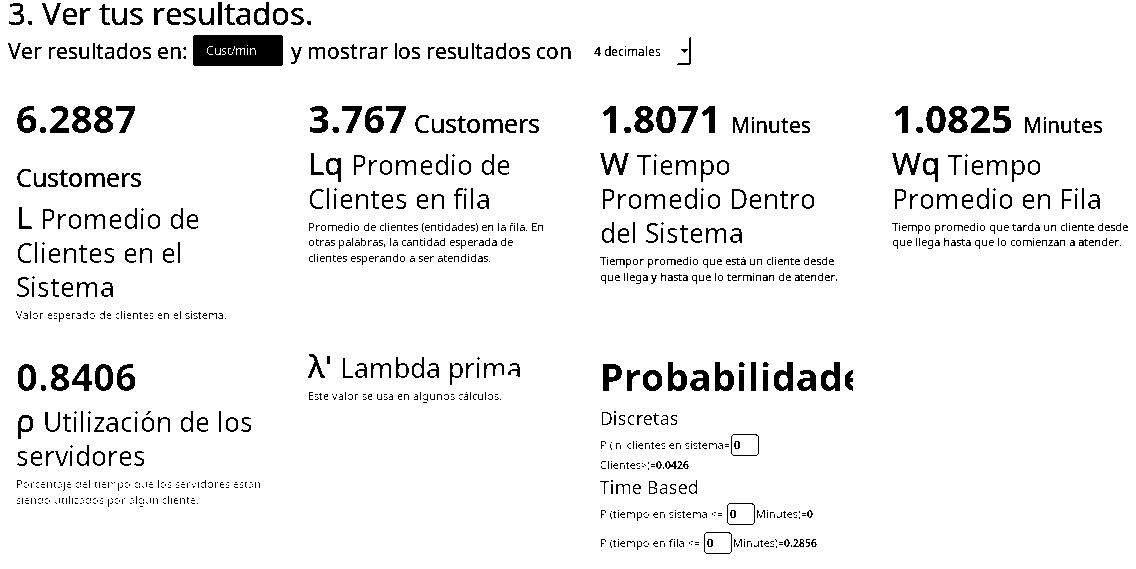
\includegraphics[scale=0.35]{./report/img/menos10/S3_resultado.png}}
	\subfigure[4 servidores]{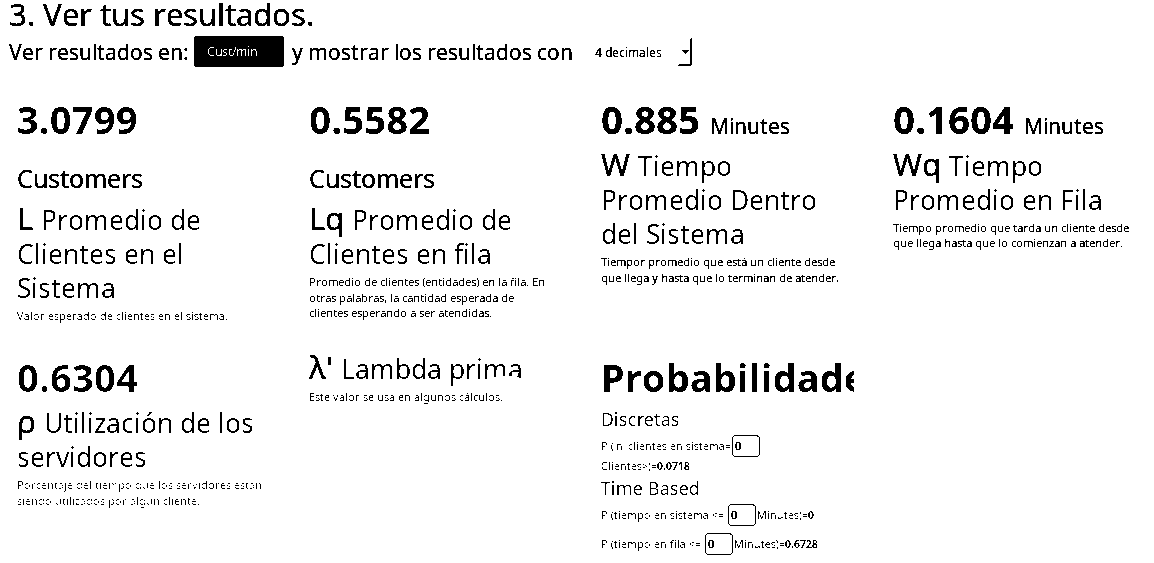
\includegraphics[scale=0.35]{./report/img/menos10/S4_resultado.png}}
	\caption{Resultados para configurações com S = 3 e S = 4 para até 10 items}
\label{fig:figure11}
\end{figure}

\begin{figure}[<+htpb+>]
	\centering
	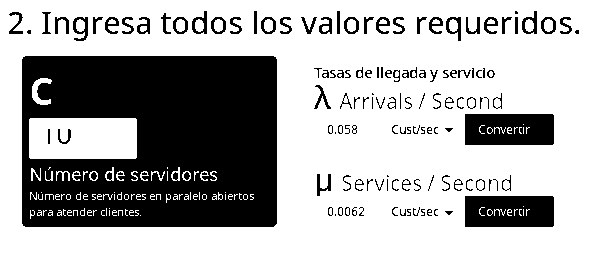
\includegraphics[scale=0.75]{./report/img/mais10/S10_valor.png}
	\caption{Valores introduzidos para a solução ótima para 10 servidores, para
	mais de 10 compras }
\label{fig:figure2}
\end{figure}

\begin{figure}[<+htpb+>]
	\centering
	\subfigure[10 serviodores]{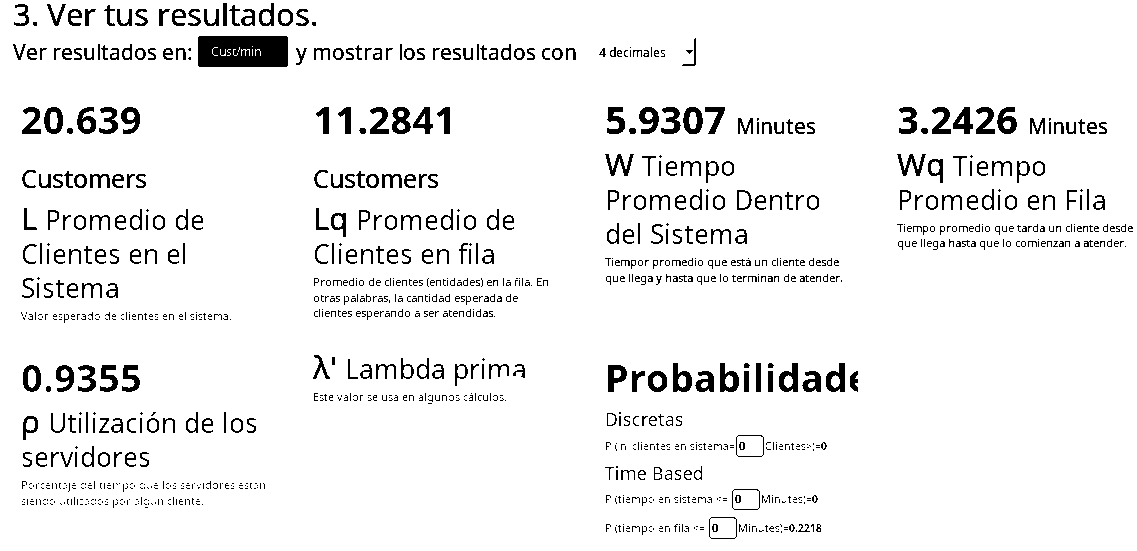
\includegraphics[scale=0.35]{./report/img/mais10/S10_resultado.png}}
	\subfigure[11 servidores]{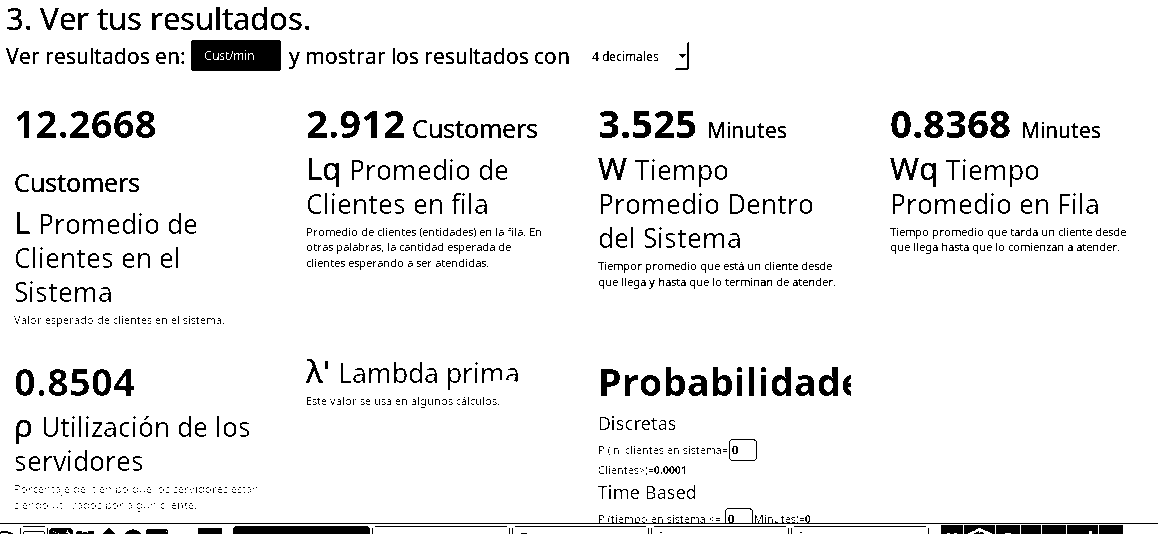
\includegraphics[scale=0.35]{./report/img/mais10/S11_resultado.png}}
	\subfigure[12 serviores] {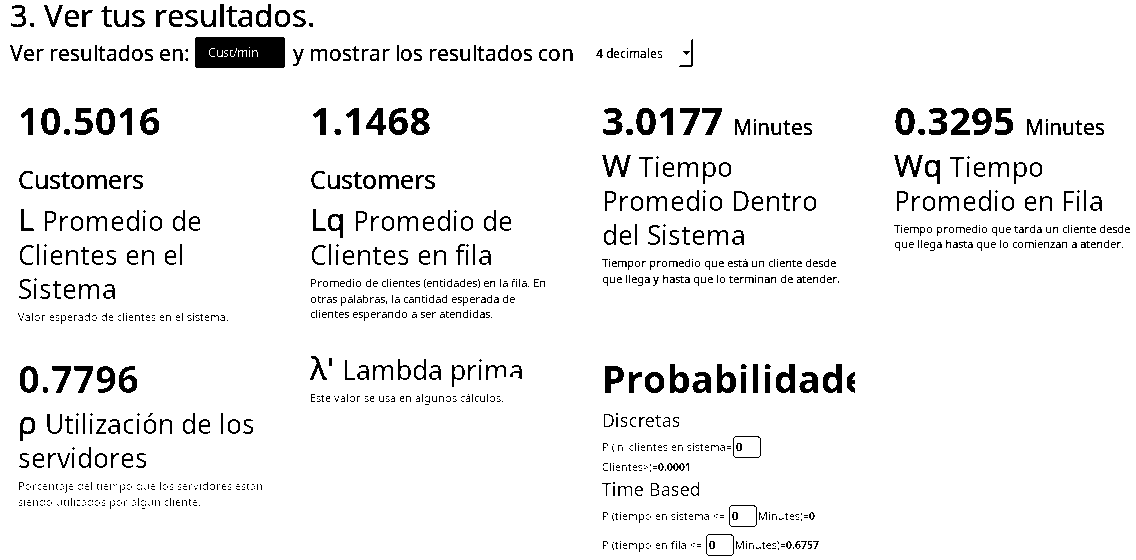
\includegraphics[scale=0.35]{./report/img/mais10/S12_resultado.png}}
	\caption{Resultados para configurações com S = 10, S = 11 e S = 12 para para
		cima de 10 items}
\label{fig:figure22}
\end{figure}











